%%%%%%%%%%%%%%%%%%%%%%%%%%%%%%

% Preamble

% The preamble does a few things:
% - Defines the type of document we want to make.
% - Loads packages which give extra tools to do things like add figures or type niche symbols
% - We can also set our own formatting rules that will be used in the main document

%%%%%%%%%%%%%%%%%%%%%%%%%%%%%%
\documentclass{article} % define the type of document. the `article' class is just about the most basic type.

\usepackage{graphicx} % Required for inserting images
\graphicspath{{./figures/}} % optional, tells LaTeX to look for images in the `figures' directory

\usepackage{amsmath} % useful for writing maths

% These are used by the \maketitle command to put in a title page/section
\title{LaTeX Tutorial}
\author{Jeremy Worsfold}
\date{\today}

%%%%%%%%%%%%%%%%%%%%%%%%%%%%%%

% Main body

% Everything in between the \begin{document} ... \end{document} commands will be put into the document in some way
% Here we write text, equations, load figures, put bibliographies and appendices
% We can use LaTeX's default commands and the ones provided by the document class and packages we loaded from the preamble
% Anything with a backslash is a command 
% Anything in the form \begin{...} \end{...} is called an environment

%%%%%%%%%%%%%%%%%%%%%%%%%%%%%%
\begin{document}

\maketitle

\section{Introduction} % the section command creates a new numbered heading 

\subsection{Smaller title} % we can also created subheadings

I can type sentences and paragraphs just by typing.
A new line doesn't do anything really but it helps you see your text easier and track changes better.
I like to start a new line for each sentence.

A blank line, however, does start a new paragraph. You can force line breaks with double backslashes but I wouldn't advise this. 
Be careful with some special characters when typing such as ampersands, percentage, dollar, at symbol etc. 
To show these as text, use a \textbackslash\; before: \%, \$, \&, \$. 
But these shouldn't come up regularly anyway.
For single quotation marks, use `at the start and' at the end. For double quotes, use ``and''. 
If you didn't, the left one would look "weird".


\begingroup % the \begingroup \endgroup means commands like \setlength are only changed for content within 

\setlength{\parskip}{1em}
I can change things like the spacing between paragraphs using \texttt{setlength}.
\texttt{1em} sets the spacing to one uppercase character's height. 
\texttt{begingroup} and \texttt{endgroup} define a region where the changes are localized. If we didn't have these, the changes would be applied everywhere after this point.

For figures, I use \texttt{.pdf} where possible (vector graphics instead of rasterized). It's also ok to use \texttt{.eps} (gets converted to \texttt{.pdf}), \texttt{.png}, potentially others like  \texttt{.jpeg}.
\begin{figure}
    \centering
    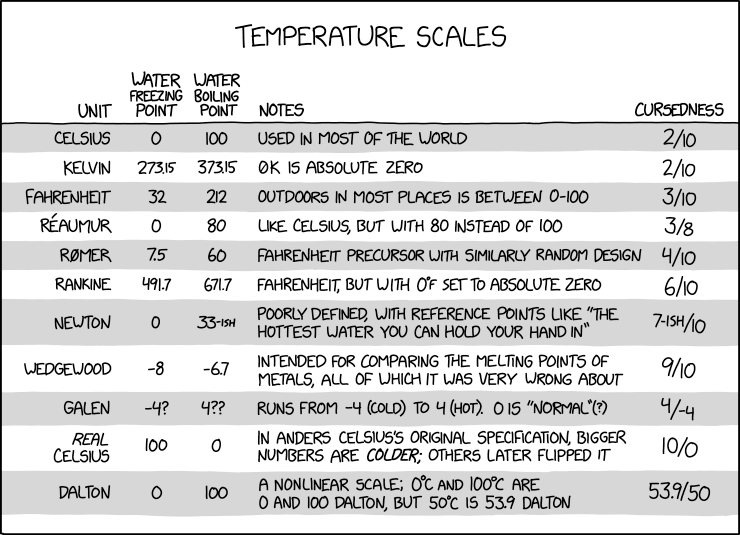
\includegraphics[width=0.8\linewidth]{temperature_scales.png}
    \caption{Make sure you write a caption.}
    \label{fig:temp-scales}
\end{figure}

\endgroup




\section{Typesetting maths}

You can add maths inline using $x=mx + b$, or \(x=mx+b\). You can put it on its own line using 
\[
    A\Sigma + \Sigma A^T = B
\]
But I typically use an equation \textit{environment}
\begin{equation}
    \int_{-\infty}^\infty e^{-x^2} d x = \sqrt{\pi}
\end{equation}
Or the same way but not with numbering
\begin{equation*}
    \int_{-\infty}^\infty e^{-ax^2} d x = \sqrt{\frac{\pi}{a}}
\end{equation*}

Importing other packages can bring other ways of typesetting maths, eg the \texttt{amsmath} package brings the \texttt{align} environment, which works the same way but also allows you to split equations across multiple lines
\begin{align}
    \sin(2\theta) & = 2\cos(\theta)\sin(\theta) \\
    & = 1-2\cos^2(\theta).
\end{align}
The double backslash starts a new line and the ampersands are the anchor points for each line.
For more information on breaking across multiple lines and and different ways of numbering, look up and have a go with other environments.
For example, using \texttt{subequations, align}:
\begin{subequations} % number equations with a,b etc
\begin{align} % allow equations to go over multiple lines
    \sin(2\theta) & = 2\cos(\theta)\sin(\theta) \\
    & = 1-2\cos^2(\theta).
\end{align}
\end{subequations}

Using \texttt{equation, aligned}:
\begin{equation} % number equations with a,b etc
\begin{aligned} % allow equations to go over multiple lines
    \sin(2\theta) & = 2\cos(\theta)\sin(\theta) \\
    & = 1-2\cos^2(\theta).
\end{aligned}
\end{equation}

\end{document}
